%% LyX 2.1.0svn created this file.  For more info, see http://www.lyx.org/.
%% Do not edit unless you really know what you are doing.
\documentclass{article}
\usepackage{graphicx, color}
\newcommand{\hlnumber}[1]{\textcolor[rgb]{0,0,0}{#1}}%
\newcommand{\hlfunctioncall}[1]{\textcolor[rgb]{.5,0,.33}{\textbf{#1}}}%
\newcommand{\hlstring}[1]{\textcolor[rgb]{.6,.6,1}{#1}}%
\newcommand{\hlkeyword}[1]{\textbf{#1}}%
\newcommand{\hlargument}[1]{\textcolor[rgb]{.69,.25,.02}{#1}}%
\newcommand{\hlcomment}[1]{\textcolor[rgb]{.18,.6,.34}{#1}}%
\newcommand{\hlroxygencomment}[1]{\textcolor[rgb]{.44,.48,.7}{#1}}%
\newcommand{\hlformalargs}[1]{\hlargument{#1}}%
\newcommand{\hleqformalargs}[1]{\hlargument{#1}}%
\newcommand{\hlassignement}[1]{\textbf{#1}}%
\newcommand{\hlpackage}[1]{\textcolor[rgb]{.59,.71,.145}{#1}}%
\newcommand{\hlslot}[1]{\textit{#1}}%
\newcommand{\hlsymbol}[1]{#1}%
\newcommand{\hlprompt}[1]{\textcolor[rgb]{.5,.5,.5}{#1}}%

\usepackage{color}%
 
\newsavebox{\hlnormalsizeboxclosebrace}%
\newsavebox{\hlnormalsizeboxopenbrace}%
\newsavebox{\hlnormalsizeboxbackslash}%
\newsavebox{\hlnormalsizeboxlessthan}%
\newsavebox{\hlnormalsizeboxgreaterthan}%
\newsavebox{\hlnormalsizeboxdollar}%
\newsavebox{\hlnormalsizeboxunderscore}%
\newsavebox{\hlnormalsizeboxand}%
\newsavebox{\hlnormalsizeboxhash}%
\newsavebox{\hlnormalsizeboxat}%
\newsavebox{\hlnormalsizeboxpercent}% 
\newsavebox{\hlnormalsizeboxhat}%
\newsavebox{\hlnormalsizeboxsinglequote}%
\newsavebox{\hlnormalsizeboxbacktick}%

\setbox\hlnormalsizeboxopenbrace=\hbox{\begin{normalsize}\verb.{.\end{normalsize}}%
\setbox\hlnormalsizeboxclosebrace=\hbox{\begin{normalsize}\verb.}.\end{normalsize}}%
\setbox\hlnormalsizeboxlessthan=\hbox{\begin{normalsize}\verb.<.\end{normalsize}}%
\setbox\hlnormalsizeboxdollar=\hbox{\begin{normalsize}\verb.$.\end{normalsize}}%
\setbox\hlnormalsizeboxunderscore=\hbox{\begin{normalsize}\verb._.\end{normalsize}}%
\setbox\hlnormalsizeboxand=\hbox{\begin{normalsize}\verb.&.\end{normalsize}}%
\setbox\hlnormalsizeboxhash=\hbox{\begin{normalsize}\verb.#.\end{normalsize}}%
\setbox\hlnormalsizeboxat=\hbox{\begin{normalsize}\verb.@.\end{normalsize}}%
\setbox\hlnormalsizeboxbackslash=\hbox{\begin{normalsize}\verb.\.\end{normalsize}}%
\setbox\hlnormalsizeboxgreaterthan=\hbox{\begin{normalsize}\verb.>.\end{normalsize}}%
\setbox\hlnormalsizeboxpercent=\hbox{\begin{normalsize}\verb.%.\end{normalsize}}%
\setbox\hlnormalsizeboxhat=\hbox{\begin{normalsize}\verb.^.\end{normalsize}}%
\setbox\hlnormalsizeboxsinglequote=\hbox{\begin{normalsize}\verb.'.\end{normalsize}}%
\setbox\hlnormalsizeboxbacktick=\hbox{\begin{normalsize}\verb.`.\end{normalsize}}%
\setbox\hlnormalsizeboxhat=\hbox{\begin{normalsize}\verb.^.\end{normalsize}}%



\newsavebox{\hltinyboxclosebrace}%
\newsavebox{\hltinyboxopenbrace}%
\newsavebox{\hltinyboxbackslash}%
\newsavebox{\hltinyboxlessthan}%
\newsavebox{\hltinyboxgreaterthan}%
\newsavebox{\hltinyboxdollar}%
\newsavebox{\hltinyboxunderscore}%
\newsavebox{\hltinyboxand}%
\newsavebox{\hltinyboxhash}%
\newsavebox{\hltinyboxat}%
\newsavebox{\hltinyboxpercent}% 
\newsavebox{\hltinyboxhat}%
\newsavebox{\hltinyboxsinglequote}%
\newsavebox{\hltinyboxbacktick}%

\setbox\hltinyboxopenbrace=\hbox{\begin{tiny}\verb.{.\end{tiny}}%
\setbox\hltinyboxclosebrace=\hbox{\begin{tiny}\verb.}.\end{tiny}}%
\setbox\hltinyboxlessthan=\hbox{\begin{tiny}\verb.<.\end{tiny}}%
\setbox\hltinyboxdollar=\hbox{\begin{tiny}\verb.$.\end{tiny}}%
\setbox\hltinyboxunderscore=\hbox{\begin{tiny}\verb._.\end{tiny}}%
\setbox\hltinyboxand=\hbox{\begin{tiny}\verb.&.\end{tiny}}%
\setbox\hltinyboxhash=\hbox{\begin{tiny}\verb.#.\end{tiny}}%
\setbox\hltinyboxat=\hbox{\begin{tiny}\verb.@.\end{tiny}}%
\setbox\hltinyboxbackslash=\hbox{\begin{tiny}\verb.\.\end{tiny}}%
\setbox\hltinyboxgreaterthan=\hbox{\begin{tiny}\verb.>.\end{tiny}}%
\setbox\hltinyboxpercent=\hbox{\begin{tiny}\verb.%.\end{tiny}}%
\setbox\hltinyboxhat=\hbox{\begin{tiny}\verb.^.\end{tiny}}%
\setbox\hltinyboxsinglequote=\hbox{\begin{tiny}\verb.'.\end{tiny}}%
\setbox\hltinyboxbacktick=\hbox{\begin{tiny}\verb.`.\end{tiny}}%
\setbox\hltinyboxhat=\hbox{\begin{tiny}\verb.^.\end{tiny}}%



\newsavebox{\hlscriptsizeboxclosebrace}%
\newsavebox{\hlscriptsizeboxopenbrace}%
\newsavebox{\hlscriptsizeboxbackslash}%
\newsavebox{\hlscriptsizeboxlessthan}%
\newsavebox{\hlscriptsizeboxgreaterthan}%
\newsavebox{\hlscriptsizeboxdollar}%
\newsavebox{\hlscriptsizeboxunderscore}%
\newsavebox{\hlscriptsizeboxand}%
\newsavebox{\hlscriptsizeboxhash}%
\newsavebox{\hlscriptsizeboxat}%
\newsavebox{\hlscriptsizeboxpercent}% 
\newsavebox{\hlscriptsizeboxhat}%
\newsavebox{\hlscriptsizeboxsinglequote}%
\newsavebox{\hlscriptsizeboxbacktick}%

\setbox\hlscriptsizeboxopenbrace=\hbox{\begin{scriptsize}\verb.{.\end{scriptsize}}%
\setbox\hlscriptsizeboxclosebrace=\hbox{\begin{scriptsize}\verb.}.\end{scriptsize}}%
\setbox\hlscriptsizeboxlessthan=\hbox{\begin{scriptsize}\verb.<.\end{scriptsize}}%
\setbox\hlscriptsizeboxdollar=\hbox{\begin{scriptsize}\verb.$.\end{scriptsize}}%
\setbox\hlscriptsizeboxunderscore=\hbox{\begin{scriptsize}\verb._.\end{scriptsize}}%
\setbox\hlscriptsizeboxand=\hbox{\begin{scriptsize}\verb.&.\end{scriptsize}}%
\setbox\hlscriptsizeboxhash=\hbox{\begin{scriptsize}\verb.#.\end{scriptsize}}%
\setbox\hlscriptsizeboxat=\hbox{\begin{scriptsize}\verb.@.\end{scriptsize}}%
\setbox\hlscriptsizeboxbackslash=\hbox{\begin{scriptsize}\verb.\.\end{scriptsize}}%
\setbox\hlscriptsizeboxgreaterthan=\hbox{\begin{scriptsize}\verb.>.\end{scriptsize}}%
\setbox\hlscriptsizeboxpercent=\hbox{\begin{scriptsize}\verb.%.\end{scriptsize}}%
\setbox\hlscriptsizeboxhat=\hbox{\begin{scriptsize}\verb.^.\end{scriptsize}}%
\setbox\hlscriptsizeboxsinglequote=\hbox{\begin{scriptsize}\verb.'.\end{scriptsize}}%
\setbox\hlscriptsizeboxbacktick=\hbox{\begin{scriptsize}\verb.`.\end{scriptsize}}%
\setbox\hlscriptsizeboxhat=\hbox{\begin{scriptsize}\verb.^.\end{scriptsize}}%



\newsavebox{\hlfootnotesizeboxclosebrace}%
\newsavebox{\hlfootnotesizeboxopenbrace}%
\newsavebox{\hlfootnotesizeboxbackslash}%
\newsavebox{\hlfootnotesizeboxlessthan}%
\newsavebox{\hlfootnotesizeboxgreaterthan}%
\newsavebox{\hlfootnotesizeboxdollar}%
\newsavebox{\hlfootnotesizeboxunderscore}%
\newsavebox{\hlfootnotesizeboxand}%
\newsavebox{\hlfootnotesizeboxhash}%
\newsavebox{\hlfootnotesizeboxat}%
\newsavebox{\hlfootnotesizeboxpercent}% 
\newsavebox{\hlfootnotesizeboxhat}%
\newsavebox{\hlfootnotesizeboxsinglequote}%
\newsavebox{\hlfootnotesizeboxbacktick}%

\setbox\hlfootnotesizeboxopenbrace=\hbox{\begin{footnotesize}\verb.{.\end{footnotesize}}%
\setbox\hlfootnotesizeboxclosebrace=\hbox{\begin{footnotesize}\verb.}.\end{footnotesize}}%
\setbox\hlfootnotesizeboxlessthan=\hbox{\begin{footnotesize}\verb.<.\end{footnotesize}}%
\setbox\hlfootnotesizeboxdollar=\hbox{\begin{footnotesize}\verb.$.\end{footnotesize}}%
\setbox\hlfootnotesizeboxunderscore=\hbox{\begin{footnotesize}\verb._.\end{footnotesize}}%
\setbox\hlfootnotesizeboxand=\hbox{\begin{footnotesize}\verb.&.\end{footnotesize}}%
\setbox\hlfootnotesizeboxhash=\hbox{\begin{footnotesize}\verb.#.\end{footnotesize}}%
\setbox\hlfootnotesizeboxat=\hbox{\begin{footnotesize}\verb.@.\end{footnotesize}}%
\setbox\hlfootnotesizeboxbackslash=\hbox{\begin{footnotesize}\verb.\.\end{footnotesize}}%
\setbox\hlfootnotesizeboxgreaterthan=\hbox{\begin{footnotesize}\verb.>.\end{footnotesize}}%
\setbox\hlfootnotesizeboxpercent=\hbox{\begin{footnotesize}\verb.%.\end{footnotesize}}%
\setbox\hlfootnotesizeboxhat=\hbox{\begin{footnotesize}\verb.^.\end{footnotesize}}%
\setbox\hlfootnotesizeboxsinglequote=\hbox{\begin{footnotesize}\verb.'.\end{footnotesize}}%
\setbox\hlfootnotesizeboxbacktick=\hbox{\begin{footnotesize}\verb.`.\end{footnotesize}}%
\setbox\hlfootnotesizeboxhat=\hbox{\begin{footnotesize}\verb.^.\end{footnotesize}}%



\newsavebox{\hlsmallboxclosebrace}%
\newsavebox{\hlsmallboxopenbrace}%
\newsavebox{\hlsmallboxbackslash}%
\newsavebox{\hlsmallboxlessthan}%
\newsavebox{\hlsmallboxgreaterthan}%
\newsavebox{\hlsmallboxdollar}%
\newsavebox{\hlsmallboxunderscore}%
\newsavebox{\hlsmallboxand}%
\newsavebox{\hlsmallboxhash}%
\newsavebox{\hlsmallboxat}%
\newsavebox{\hlsmallboxpercent}% 
\newsavebox{\hlsmallboxhat}%
\newsavebox{\hlsmallboxsinglequote}%
\newsavebox{\hlsmallboxbacktick}%

\setbox\hlsmallboxopenbrace=\hbox{\begin{small}\verb.{.\end{small}}%
\setbox\hlsmallboxclosebrace=\hbox{\begin{small}\verb.}.\end{small}}%
\setbox\hlsmallboxlessthan=\hbox{\begin{small}\verb.<.\end{small}}%
\setbox\hlsmallboxdollar=\hbox{\begin{small}\verb.$.\end{small}}%
\setbox\hlsmallboxunderscore=\hbox{\begin{small}\verb._.\end{small}}%
\setbox\hlsmallboxand=\hbox{\begin{small}\verb.&.\end{small}}%
\setbox\hlsmallboxhash=\hbox{\begin{small}\verb.#.\end{small}}%
\setbox\hlsmallboxat=\hbox{\begin{small}\verb.@.\end{small}}%
\setbox\hlsmallboxbackslash=\hbox{\begin{small}\verb.\.\end{small}}%
\setbox\hlsmallboxgreaterthan=\hbox{\begin{small}\verb.>.\end{small}}%
\setbox\hlsmallboxpercent=\hbox{\begin{small}\verb.%.\end{small}}%
\setbox\hlsmallboxhat=\hbox{\begin{small}\verb.^.\end{small}}%
\setbox\hlsmallboxsinglequote=\hbox{\begin{small}\verb.'.\end{small}}%
\setbox\hlsmallboxbacktick=\hbox{\begin{small}\verb.`.\end{small}}%
\setbox\hlsmallboxhat=\hbox{\begin{small}\verb.^.\end{small}}%



\newsavebox{\hllargeboxclosebrace}%
\newsavebox{\hllargeboxopenbrace}%
\newsavebox{\hllargeboxbackslash}%
\newsavebox{\hllargeboxlessthan}%
\newsavebox{\hllargeboxgreaterthan}%
\newsavebox{\hllargeboxdollar}%
\newsavebox{\hllargeboxunderscore}%
\newsavebox{\hllargeboxand}%
\newsavebox{\hllargeboxhash}%
\newsavebox{\hllargeboxat}%
\newsavebox{\hllargeboxpercent}% 
\newsavebox{\hllargeboxhat}%
\newsavebox{\hllargeboxsinglequote}%
\newsavebox{\hllargeboxbacktick}%

\setbox\hllargeboxopenbrace=\hbox{\begin{large}\verb.{.\end{large}}%
\setbox\hllargeboxclosebrace=\hbox{\begin{large}\verb.}.\end{large}}%
\setbox\hllargeboxlessthan=\hbox{\begin{large}\verb.<.\end{large}}%
\setbox\hllargeboxdollar=\hbox{\begin{large}\verb.$.\end{large}}%
\setbox\hllargeboxunderscore=\hbox{\begin{large}\verb._.\end{large}}%
\setbox\hllargeboxand=\hbox{\begin{large}\verb.&.\end{large}}%
\setbox\hllargeboxhash=\hbox{\begin{large}\verb.#.\end{large}}%
\setbox\hllargeboxat=\hbox{\begin{large}\verb.@.\end{large}}%
\setbox\hllargeboxbackslash=\hbox{\begin{large}\verb.\.\end{large}}%
\setbox\hllargeboxgreaterthan=\hbox{\begin{large}\verb.>.\end{large}}%
\setbox\hllargeboxpercent=\hbox{\begin{large}\verb.%.\end{large}}%
\setbox\hllargeboxhat=\hbox{\begin{large}\verb.^.\end{large}}%
\setbox\hllargeboxsinglequote=\hbox{\begin{large}\verb.'.\end{large}}%
\setbox\hllargeboxbacktick=\hbox{\begin{large}\verb.`.\end{large}}%
\setbox\hllargeboxhat=\hbox{\begin{large}\verb.^.\end{large}}%



\newsavebox{\hlLargeboxclosebrace}%
\newsavebox{\hlLargeboxopenbrace}%
\newsavebox{\hlLargeboxbackslash}%
\newsavebox{\hlLargeboxlessthan}%
\newsavebox{\hlLargeboxgreaterthan}%
\newsavebox{\hlLargeboxdollar}%
\newsavebox{\hlLargeboxunderscore}%
\newsavebox{\hlLargeboxand}%
\newsavebox{\hlLargeboxhash}%
\newsavebox{\hlLargeboxat}%
\newsavebox{\hlLargeboxpercent}% 
\newsavebox{\hlLargeboxhat}%
\newsavebox{\hlLargeboxsinglequote}%
\newsavebox{\hlLargeboxbacktick}%

\setbox\hlLargeboxopenbrace=\hbox{\begin{Large}\verb.{.\end{Large}}%
\setbox\hlLargeboxclosebrace=\hbox{\begin{Large}\verb.}.\end{Large}}%
\setbox\hlLargeboxlessthan=\hbox{\begin{Large}\verb.<.\end{Large}}%
\setbox\hlLargeboxdollar=\hbox{\begin{Large}\verb.$.\end{Large}}%
\setbox\hlLargeboxunderscore=\hbox{\begin{Large}\verb._.\end{Large}}%
\setbox\hlLargeboxand=\hbox{\begin{Large}\verb.&.\end{Large}}%
\setbox\hlLargeboxhash=\hbox{\begin{Large}\verb.#.\end{Large}}%
\setbox\hlLargeboxat=\hbox{\begin{Large}\verb.@.\end{Large}}%
\setbox\hlLargeboxbackslash=\hbox{\begin{Large}\verb.\.\end{Large}}%
\setbox\hlLargeboxgreaterthan=\hbox{\begin{Large}\verb.>.\end{Large}}%
\setbox\hlLargeboxpercent=\hbox{\begin{Large}\verb.%.\end{Large}}%
\setbox\hlLargeboxhat=\hbox{\begin{Large}\verb.^.\end{Large}}%
\setbox\hlLargeboxsinglequote=\hbox{\begin{Large}\verb.'.\end{Large}}%
\setbox\hlLargeboxbacktick=\hbox{\begin{Large}\verb.`.\end{Large}}%
\setbox\hlLargeboxhat=\hbox{\begin{Large}\verb.^.\end{Large}}%



\newsavebox{\hlLARGEboxclosebrace}%
\newsavebox{\hlLARGEboxopenbrace}%
\newsavebox{\hlLARGEboxbackslash}%
\newsavebox{\hlLARGEboxlessthan}%
\newsavebox{\hlLARGEboxgreaterthan}%
\newsavebox{\hlLARGEboxdollar}%
\newsavebox{\hlLARGEboxunderscore}%
\newsavebox{\hlLARGEboxand}%
\newsavebox{\hlLARGEboxhash}%
\newsavebox{\hlLARGEboxat}%
\newsavebox{\hlLARGEboxpercent}% 
\newsavebox{\hlLARGEboxhat}%
\newsavebox{\hlLARGEboxsinglequote}%
\newsavebox{\hlLARGEboxbacktick}%

\setbox\hlLARGEboxopenbrace=\hbox{\begin{LARGE}\verb.{.\end{LARGE}}%
\setbox\hlLARGEboxclosebrace=\hbox{\begin{LARGE}\verb.}.\end{LARGE}}%
\setbox\hlLARGEboxlessthan=\hbox{\begin{LARGE}\verb.<.\end{LARGE}}%
\setbox\hlLARGEboxdollar=\hbox{\begin{LARGE}\verb.$.\end{LARGE}}%
\setbox\hlLARGEboxunderscore=\hbox{\begin{LARGE}\verb._.\end{LARGE}}%
\setbox\hlLARGEboxand=\hbox{\begin{LARGE}\verb.&.\end{LARGE}}%
\setbox\hlLARGEboxhash=\hbox{\begin{LARGE}\verb.#.\end{LARGE}}%
\setbox\hlLARGEboxat=\hbox{\begin{LARGE}\verb.@.\end{LARGE}}%
\setbox\hlLARGEboxbackslash=\hbox{\begin{LARGE}\verb.\.\end{LARGE}}%
\setbox\hlLARGEboxgreaterthan=\hbox{\begin{LARGE}\verb.>.\end{LARGE}}%
\setbox\hlLARGEboxpercent=\hbox{\begin{LARGE}\verb.%.\end{LARGE}}%
\setbox\hlLARGEboxhat=\hbox{\begin{LARGE}\verb.^.\end{LARGE}}%
\setbox\hlLARGEboxsinglequote=\hbox{\begin{LARGE}\verb.'.\end{LARGE}}%
\setbox\hlLARGEboxbacktick=\hbox{\begin{LARGE}\verb.`.\end{LARGE}}%
\setbox\hlLARGEboxhat=\hbox{\begin{LARGE}\verb.^.\end{LARGE}}%



\newsavebox{\hlhugeboxclosebrace}%
\newsavebox{\hlhugeboxopenbrace}%
\newsavebox{\hlhugeboxbackslash}%
\newsavebox{\hlhugeboxlessthan}%
\newsavebox{\hlhugeboxgreaterthan}%
\newsavebox{\hlhugeboxdollar}%
\newsavebox{\hlhugeboxunderscore}%
\newsavebox{\hlhugeboxand}%
\newsavebox{\hlhugeboxhash}%
\newsavebox{\hlhugeboxat}%
\newsavebox{\hlhugeboxpercent}% 
\newsavebox{\hlhugeboxhat}%
\newsavebox{\hlhugeboxsinglequote}%
\newsavebox{\hlhugeboxbacktick}%

\setbox\hlhugeboxopenbrace=\hbox{\begin{huge}\verb.{.\end{huge}}%
\setbox\hlhugeboxclosebrace=\hbox{\begin{huge}\verb.}.\end{huge}}%
\setbox\hlhugeboxlessthan=\hbox{\begin{huge}\verb.<.\end{huge}}%
\setbox\hlhugeboxdollar=\hbox{\begin{huge}\verb.$.\end{huge}}%
\setbox\hlhugeboxunderscore=\hbox{\begin{huge}\verb._.\end{huge}}%
\setbox\hlhugeboxand=\hbox{\begin{huge}\verb.&.\end{huge}}%
\setbox\hlhugeboxhash=\hbox{\begin{huge}\verb.#.\end{huge}}%
\setbox\hlhugeboxat=\hbox{\begin{huge}\verb.@.\end{huge}}%
\setbox\hlhugeboxbackslash=\hbox{\begin{huge}\verb.\.\end{huge}}%
\setbox\hlhugeboxgreaterthan=\hbox{\begin{huge}\verb.>.\end{huge}}%
\setbox\hlhugeboxpercent=\hbox{\begin{huge}\verb.%.\end{huge}}%
\setbox\hlhugeboxhat=\hbox{\begin{huge}\verb.^.\end{huge}}%
\setbox\hlhugeboxsinglequote=\hbox{\begin{huge}\verb.'.\end{huge}}%
\setbox\hlhugeboxbacktick=\hbox{\begin{huge}\verb.`.\end{huge}}%
\setbox\hlhugeboxhat=\hbox{\begin{huge}\verb.^.\end{huge}}%



\newsavebox{\hlHugeboxclosebrace}%
\newsavebox{\hlHugeboxopenbrace}%
\newsavebox{\hlHugeboxbackslash}%
\newsavebox{\hlHugeboxlessthan}%
\newsavebox{\hlHugeboxgreaterthan}%
\newsavebox{\hlHugeboxdollar}%
\newsavebox{\hlHugeboxunderscore}%
\newsavebox{\hlHugeboxand}%
\newsavebox{\hlHugeboxhash}%
\newsavebox{\hlHugeboxat}%
\newsavebox{\hlHugeboxpercent}% 
\newsavebox{\hlHugeboxhat}%
\newsavebox{\hlHugeboxsinglequote}%
\newsavebox{\hlHugeboxbacktick}%

\setbox\hlHugeboxopenbrace=\hbox{\begin{Huge}\verb.{.\end{Huge}}%
\setbox\hlHugeboxclosebrace=\hbox{\begin{Huge}\verb.}.\end{Huge}}%
\setbox\hlHugeboxlessthan=\hbox{\begin{Huge}\verb.<.\end{Huge}}%
\setbox\hlHugeboxdollar=\hbox{\begin{Huge}\verb.$.\end{Huge}}%
\setbox\hlHugeboxunderscore=\hbox{\begin{Huge}\verb._.\end{Huge}}%
\setbox\hlHugeboxand=\hbox{\begin{Huge}\verb.&.\end{Huge}}%
\setbox\hlHugeboxhash=\hbox{\begin{Huge}\verb.#.\end{Huge}}%
\setbox\hlHugeboxat=\hbox{\begin{Huge}\verb.@.\end{Huge}}%
\setbox\hlHugeboxbackslash=\hbox{\begin{Huge}\verb.\.\end{Huge}}%
\setbox\hlHugeboxgreaterthan=\hbox{\begin{Huge}\verb.>.\end{Huge}}%
\setbox\hlHugeboxpercent=\hbox{\begin{Huge}\verb.%.\end{Huge}}%
\setbox\hlHugeboxhat=\hbox{\begin{Huge}\verb.^.\end{Huge}}%
\setbox\hlHugeboxsinglequote=\hbox{\begin{Huge}\verb.'.\end{Huge}}%
\setbox\hlHugeboxbacktick=\hbox{\begin{Huge}\verb.`.\end{Huge}}%
\setbox\hlHugeboxhat=\hbox{\begin{Huge}\verb.^.\end{Huge}}%
 

\def\urltilda{\kern -.15em\lower .7ex\hbox{\~{}}\kern .04em}%

\newcommand{\hlstd}[1]{\textcolor[rgb]{0,0,0}{#1}}%
\newcommand{\hlnum}[1]{\textcolor[rgb]{0.16,0.16,1}{#1}}
\newcommand{\hlesc}[1]{\textcolor[rgb]{1,0,1}{#1}}
\newcommand{\hlstr}[1]{\textcolor[rgb]{1,0,0}{#1}}
\newcommand{\hldstr}[1]{\textcolor[rgb]{0.51,0.51,0}{#1}}
\newcommand{\hlslc}[1]{\textcolor[rgb]{0.51,0.51,0.51}{\it{#1}}}
\newcommand{\hlcom}[1]{\textcolor[rgb]{0.51,0.51,0.51}{\it{#1}}}
\newcommand{\hldir}[1]{\textcolor[rgb]{0,0.51,0}{#1}}
\newcommand{\hlsym}[1]{\textcolor[rgb]{0,0,0}{#1}}
\newcommand{\hlline}[1]{\textcolor[rgb]{0.33,0.33,0.33}{#1}}
\newcommand{\hlkwa}[1]{\textcolor[rgb]{0,0,0}{\bf{#1}}}
\newcommand{\hlkwb}[1]{\textcolor[rgb]{0.51,0,0}{#1}}
\newcommand{\hlkwc}[1]{\textcolor[rgb]{0,0,0}{\bf{#1}}}
\newcommand{\hlkwd}[1]{\textcolor[rgb]{0,0,0.51}{#1}}

\definecolor{fgcolor}{rgb}{0,0,0}
\usepackage{framed}
\makeatletter
\newenvironment{kframe}{%
 \def\FrameCommand##1{\hskip\@totalleftmargin \hskip-\fboxsep
 \colorbox{shadecolor}{##1}\hskip-\fboxsep
     % There is no \@totalrightmargin, so:
     \hskip-\linewidth \hskip-\@totalleftmargin \hskip\columnwidth}%
 \MakeFramed {\advance\hsize-\width
   \@totalleftmargin\z@ \linewidth\hsize
   \@setminipage}}%
 {\par\unskip\endMakeFramed}
\makeatother

\newenvironment{knitrout}{}{} % an empty environment to be redefined in TeX

\usepackage[sc]{mathpazo}
\usepackage[T1]{fontenc}
\usepackage{geometry}
\usepackage{amssymb}
\usepackage{amsmath}
\geometry{verbose,tmargin=2.5cm,bmargin=2.5cm,lmargin=2.5cm,rmargin=2.5cm}
\setcounter{secnumdepth}{2}
\setcounter{tocdepth}{2}
\usepackage{url}
\usepackage[unicode=true,pdfusetitle,
 bookmarks=true,bookmarksnumbered=true,bookmarksopen=true,bookmarksopenlevel=2,
 breaklinks=false,pdfborder={0 0 1},backref=false,colorlinks=false]
 {hyperref}
\hypersetup{
 pdfstartview={XYZ null null 1}}
%\usepackage{breakurl}

\makeatletter
%%%%%%%%%%%%%%%%%%%%%%%%%%%%%% User specified LaTeX commands.
\renewcommand{\textfraction}{0.05}
\renewcommand{\topfraction}{0.8}
\renewcommand{\bottomfraction}{0.8}
\renewcommand{\floatpagefraction}{0.75}

\makeatother

\begin{document}

% 







\begin{center}
  {\bf \Large Homework 2, Statistical Rethinking}\\
\vspace{12pt}
   {\large Jaime Ashander}
\end{center}


\subsection*{Problem 1}
\label{problem1}

First load the data from last week, \texttt{birth1} and \texttt{birth2}, which indicate the gender (male=1, female=0) of reported first (second) born children in 100 families.
All families in this country have a maximum of two children.

Our hypothesis is that births are determined by a random process, with some probability of obtaining a boy \texttt{p.b}.
Assuming births are independent samples of this process, we model the data as random binomial trials.

\subsubsection*{1 a}
\label{1a}

Now we will compute a $p$ value for $H_0$:  {\tt p.b = 0.5}.
That is, we compute the probability we would see a result as deviant (or more deviant) assuming the null is true.

\begin{knitrout}
\definecolor{shadecolor}{rgb}{.97, .97, .97}{\color{fgcolor}\begin{kframe}
\begin{flushleft}
\ttfamily\noindent
\hlfunctioncall{data}\hlkeyword{(}\hlsymbol{homeworkch2}\hlkeyword{)}{\ }{\ }\hlcomment{\usebox{\hlnormalsizeboxhash}}\hspace*{\fill}\\
\hlstd{}\hlsymbol{boys.born}{\ }\hlassignement{\usebox{\hlnormalsizeboxlessthan}-}{\ }\hlfunctioncall{sum}\hlkeyword{(}\hlfunctioncall{c}\hlkeyword{(}\hlsymbol{birth1}\hlkeyword{,}{\ }\hlsymbol{birth2}\hlkeyword{)}\hlkeyword{)}\hspace*{\fill}\\
\hlstd{}\hlsymbol{total.births}{\ }\hlassignement{\usebox{\hlnormalsizeboxlessthan}-}{\ }\hlfunctioncall{length}\hlkeyword{(}\hlfunctioncall{c}\hlkeyword{(}\hlsymbol{birth1}\hlkeyword{,}{\ }\hlsymbol{birth2}\hlkeyword{)}\hlkeyword{)}\hspace*{\fill}\\
\hlstd{}\hlsymbol{pb.h0}{\ }\hlassignement{\usebox{\hlnormalsizeboxlessthan}-}{\ }\hlnumber{0.5}{\ }{\ }\hlcomment{\usebox{\hlnormalsizeboxhash}0th{\ }step:{\ }specify{\ }the{\ }null}\hspace*{\fill}\\
\hlstd{}\hlsymbol{pb.mle}{\ }\hlassignement{\usebox{\hlnormalsizeboxlessthan}-}{\ }\hlsymbol{boys.born}\hlkeyword{/}\hlsymbol{total.births}{\ }{\ }\hlcomment{\usebox{\hlnormalsizeboxhash}{\ }first{\ }step:{\ }compute{\ }the{\ }observed{\ }MLE{\ }of{\ }p.b{\ }which{\ }in{\ }this{\ }case{\ }is{\ }just{\ }the{\ }proportion{\ }of{\ }boy{\ }births{\ }(more{\ }generally{\ }we{\ }could{\ }compute{\ }P(D{\ }|{\ }M){\ }assuming{\ }we{\ }could{\ }writedown{\ }the{\ }likelihood}\hspace*{\fill}\\
\hlstd{}\hlcomment{\usebox{\hlnormalsizeboxhash}{\ }second{\ }step:{\ }compute{\ }the{\ }probability{\ }of{\ }observing{\ }a{\ }range{\ }of}\hspace*{\fill}\\
\hlstd{}\hlcomment{\usebox{\hlnormalsizeboxhash}{\ }{\ }{\ }possible{\ }boys{\ }born{\ }from{\ }0{\ }to{\ }totalbirths{\ }(roughly{\ }implying}\hspace*{\fill}\\
\hlstd{}\hlcomment{\usebox{\hlnormalsizeboxhash}{\ }{\ }{\ }pb.mle{\ }from{\ }0{\ }to{\ }1){\ }\usebox{\hlnormalsizeboxunderscore}if{\ }the{\ }null{\ }were{\ }true\usebox{\hlnormalsizeboxunderscore}}\hspace*{\fill}\\
\hlstd{}\hlsymbol{p.b.observing}{\ }\hlassignement{\usebox{\hlnormalsizeboxlessthan}-}{\ }\hlfunctioncall{dbinom}\hlkeyword{(}\hlsymbol{boys.born}\hlkeyword{:}\hlsymbol{total.births}\hlkeyword{,}{\ }\hlargument{size}{\ }\hlargument{=}{\ }\hlsymbol{total.births}\hlkeyword{,}\hspace*{\fill}\\
\hlstd{}{\ }{\ }{\ }{\ }\hlargument{prob}{\ }\hlargument{=}{\ }\hlsymbol{pb.h0}\hlkeyword{)}\hspace*{\fill}\\
\hlstd{}\hlcomment{\usebox{\hlnormalsizeboxhash}{\ }third{\ }step:{\ }compute{\ }the{\ }p{\ }value{\ }by{\ }\usebox{\hlnormalsizeboxsinglequote}summing{\ }over{\ }the{\ }tail\usebox{\hlnormalsizeboxsinglequote}{\ }of}\hspace*{\fill}\\
\hlstd{}\hlcomment{\usebox{\hlnormalsizeboxhash}{\ }{\ }{\ }possible{\ }boys{\ }as{\ }great{\ }or{\ }greater{\ }(111{\ }to{\ }200)}\hspace*{\fill}\\
\hlstd{}\hlsymbol{pb.pval}{\ }\hlassignement{\usebox{\hlnormalsizeboxlessthan}-}{\ }\hlfunctioncall{sum}\hlkeyword{(}\hlsymbol{p.b.observing}\hlkeyword{)}\hspace*{\fill}\\
\hlstd{}\hlsymbol{pb.pval}\mbox{}
\normalfont
\end{flushleft}
\begin{verbatim}
## [1] 0.06868
\end{verbatim}
\end{kframe}}
\end{knitrout}


With $p > 0.05$, NHST suggests that we should fail to reject the null, in effect concluding that {\tt p.b = 0.5}.

\subsubsection*{1 b}
\label{1b}

The figure below reproduces the posterior from last week. The red line is {\tt p.b = 0.5}. 
In the context of our estimated posterior, the null is not a great point estimate to choose.
Although it does fall within the 90\% HPDI  (not shown) it falls outside the 50\% HPDI.

\begin{knitrout}
\definecolor{shadecolor}{rgb}{.97, .97, .97}{\color{fgcolor}\begin{kframe}
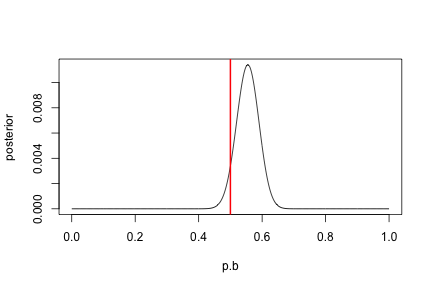
\includegraphics{null-v-prior} \end{kframe}}
\end{knitrout}



\subsection*{Problem 2}
\label{problem2}


The question: is a die loaded such that $Pr(die =1) = 1/2$ instead of typical $Pr(die=1) = 1/6$?

The data: 65 tosses, with 18 ``1''s. 

We model the data as random binomial trials, with the rolls assumed independent. 
Define a roll of 1 as a success, and let the probabilty of success {\tt p.d}. 

\begin{knitrout}
\definecolor{shadecolor}{rgb}{.97, .97, .97}{\color{fgcolor}\begin{kframe}
\begin{flushleft}
\ttfamily\noindent
\hlsymbol{die.succ}{\ }\hlassignement{\usebox{\hlnormalsizeboxlessthan}-}{\ }\hlnumber{18}\hspace*{\fill}\\
\hlstd{}\hlsymbol{die.trials}{\ }\hlassignement{\usebox{\hlnormalsizeboxlessthan}-}{\ }\hlnumber{65}\mbox{}
\normalfont
\end{flushleft}
\end{kframe}}
\end{knitrout}



\subsubsection*{2a}
\label{2a}

Using null hypotehsis signficance test, we compare the observed data against a null hypothesis: 

$H_0: p.d = 1/6$

As in Problem 1, we compute the $p$ value by assuming the null: 

\begin{knitrout}
\definecolor{shadecolor}{rgb}{.97, .97, .97}{\color{fgcolor}\begin{kframe}
\begin{flushleft}
\ttfamily\noindent
\hlsymbol{pd.h0}{\ }\hlassignement{\usebox{\hlnormalsizeboxlessthan}-}{\ }\hlnumber{1}\hlkeyword{/}\hlnumber{6}\hspace*{\fill}\\
\hlstd{}\hlsymbol{pd.mle}{\ }\hlassignement{\usebox{\hlnormalsizeboxlessthan}-}{\ }\hlsymbol{die.succ}\hlkeyword{/}\hlsymbol{die.trials}\hspace*{\fill}\\
\hlstd{}\hlsymbol{pd.under.null}{\ }\hlassignement{\usebox{\hlnormalsizeboxlessthan}-}{\ }\hlfunctioncall{dbinom}\hlkeyword{(}\hlsymbol{die.succ}\hlkeyword{:}\hlsymbol{die.trials}\hlkeyword{,}{\ }\hlargument{size}{\ }\hlargument{=}{\ }\hlsymbol{die.trials}\hlkeyword{,}\hspace*{\fill}\\
\hlstd{}{\ }{\ }{\ }{\ }\hlargument{prob}{\ }\hlargument{=}{\ }\hlsymbol{pd.h0}\hlkeyword{)}\hspace*{\fill}\\
\hlstd{}\hlsymbol{pd.pval}{\ }\hlassignement{\usebox{\hlnormalsizeboxlessthan}-}{\ }\hlfunctioncall{sum}\hlkeyword{(}\hlsymbol{pd.under.null}\hlkeyword{)}\hspace*{\fill}\\
\hlstd{}\hlsymbol{pd.pval}\mbox{}
\normalfont
\end{flushleft}
\begin{verbatim}
## [1] 0.01752
\end{verbatim}
\end{kframe}}
\end{knitrout}


With $p = 0.017< 0.05$, NHST suggests we should reject the null in favor of the alternative hypothesis: {\tt p.d > 1/6}. 

So the die is not fair!

\subsubsection*{2b}

To use the Bayesian suggestion, we apply Bayes' theorem.

\[
Pr( fair | data)  = \frac{Pr(data | fair)Pr(fair)}{Pr(data|fair)Pr(fair)+ Pr(data|loaded)Pr(loaded)}
\]

Here, as before, the data are 18 rolls of ``1'' in 65 tries.

\begin{knitrout}
\definecolor{shadecolor}{rgb}{.97, .97, .97}{\color{fgcolor}\begin{kframe}
\begin{flushleft}
\ttfamily\noindent
\hlsymbol{pd.fair}{\ }\hlassignement{\usebox{\hlnormalsizeboxlessthan}-}{\ }\hlnumber{1}\hlkeyword{/}\hlnumber{6}\hspace*{\fill}\\
\hlstd{}\hlsymbol{pd.loaded}{\ }\hlassignement{\usebox{\hlnormalsizeboxlessthan}-}{\ }\hlnumber{0.5}\hspace*{\fill}\\
\hlstd{}\hlsymbol{pr.fair}{\ }\hlassignement{\usebox{\hlnormalsizeboxlessthan}-}{\ }\hlsymbol{pr.loaded}{\ }\hlassignement{\usebox{\hlnormalsizeboxlessthan}-}{\ }\hlnumber{0.5}\hspace*{\fill}\\
\hlstd{}\hlsymbol{pr.data\usebox{\hlnormalsizeboxunderscore}fair}{\ }\hlassignement{\usebox{\hlnormalsizeboxlessthan}-}{\ }\hlfunctioncall{dbinom}\hlkeyword{(}\hlsymbol{die.succ}\hlkeyword{,}{\ }\hlargument{size}{\ }\hlargument{=}{\ }\hlsymbol{die.trials}\hlkeyword{,}{\ }\hlargument{prob}{\ }\hlargument{=}{\ }\hlsymbol{pd.fair}\hlkeyword{)}\hspace*{\fill}\\
\hlstd{}\hlsymbol{pr.data\usebox{\hlnormalsizeboxunderscore}loaded}{\ }\hlassignement{\usebox{\hlnormalsizeboxlessthan}-}{\ }\hlfunctioncall{dbinom}\hlkeyword{(}\hlsymbol{die.succ}\hlkeyword{,}{\ }\hlargument{size}{\ }\hlargument{=}{\ }\hlsymbol{die.trials}\hlkeyword{,}{\ }\hlargument{prob}{\ }\hlargument{=}{\ }\hlsymbol{pd.loaded}\hlkeyword{)}\hspace*{\fill}\\
\hlstd{}\hlsymbol{pr.data}{\ }\hlassignement{\usebox{\hlnormalsizeboxlessthan}-}{\ }\hlsymbol{pr.data\usebox{\hlnormalsizeboxunderscore}fair}{\ }\hlkeyword{*}{\ }\hlsymbol{pr.fair}{\ }\hlkeyword{+}{\ }\hlsymbol{pr.data\usebox{\hlnormalsizeboxunderscore}loaded}{\ }\hlkeyword{*}{\ }\hlsymbol{pr.loaded}\hspace*{\fill}\\
\hlstd{}\hlsymbol{pr.fair\usebox{\hlnormalsizeboxunderscore}data}{\ }\hlassignement{\usebox{\hlnormalsizeboxlessthan}-}{\ }\hlsymbol{pr.data\usebox{\hlnormalsizeboxunderscore}fair}{\ }\hlkeyword{*}{\ }\hlsymbol{pr.fair}\hlkeyword{/}\hlsymbol{pr.data}\hspace*{\fill}\\
\hlstd{}\hlsymbol{pr.fair\usebox{\hlnormalsizeboxunderscore}data}\mbox{}
\normalfont
\end{flushleft}
\begin{verbatim}
## [1] 0.9857
\end{verbatim}
\begin{flushleft}
\ttfamily\noindent
\hlnumber{18}\hlkeyword{/}\hlnumber{65}\mbox{}
\normalfont
\end{flushleft}
\begin{verbatim}
## [1] 0.2769
\end{verbatim}
\end{kframe}}
\end{knitrout}



By this analysis, there is $\approx 0.98$ probability that the die is fair. 
Quite a different result than NHST. 
If we're assuming only these two models, we should conclude the die is fair (if we're willing to risk a 2\% chance of being wrong.

But we still have reason to be nervous. 
This test and the one from part (a) are not the same. 
NHST tests fair against everything else while the Bayesian procedure tests fair against one value of loaded. 
So we should be cautious in accepting the Bayesian result uncrticially.

To assess how our observation compares to expected variabilty under our inference about the die,  we can use posterior predictive simulation.



\begin{knitrout}
\definecolor{shadecolor}{rgb}{.97, .97, .97}{\color{fgcolor}\begin{kframe}
\begin{flushleft}
\ttfamily\noindent
\hlsymbol{prob.samples}{\ }\hlassignement{\usebox{\hlnormalsizeboxlessthan}-}{\ }\hlfunctioncall{sample}\hlkeyword{(}\hlfunctioncall{c}\hlkeyword{(}\hlnumber{1}\hlkeyword{/}\hlnumber{6}\hlkeyword{,}{\ }\hlnumber{1}\hlkeyword{/}\hlnumber{2}\hlkeyword{)}\hlkeyword{,}{\ }\hlargument{size}{\ }\hlargument{=}{\ }\hlnumber{1e+06}\hlkeyword{,}{\ }\hlargument{replace}{\ }\hlargument{=}{\ }\hlnumber{TRUE}\hlkeyword{,}\hspace*{\fill}\\
\hlstd{}{\ }{\ }{\ }{\ }\hlargument{prob}{\ }\hlargument{=}{\ }\hlfunctioncall{c}\hlkeyword{(}\hlsymbol{pr.fair\usebox{\hlnormalsizeboxunderscore}data}\hlkeyword{,}{\ }\hlnumber{1}{\ }\hlkeyword{-}{\ }\hlsymbol{pr.fair\usebox{\hlnormalsizeboxunderscore}data}\hlkeyword{)}\hlkeyword{)}\hspace*{\fill}\\
\hlstd{}\hlsymbol{ones.sims}{\ }\hlassignement{\usebox{\hlnormalsizeboxlessthan}-}{\ }\hlfunctioncall{rbinom}\hlkeyword{(}\hlnumber{1e+06}\hlkeyword{,}{\ }\hlargument{size}{\ }\hlargument{=}{\ }\hlsymbol{die.trials}\hlkeyword{,}{\ }\hlargument{prob}{\ }\hlargument{=}{\ }\hlsymbol{prob.samples}\hlkeyword{)}\hspace*{\fill}\\
\hlstd{}\hlfunctioncall{dens}\hlkeyword{(}\hlsymbol{ones.sims}\hlkeyword{,}{\ }\hlargument{adj}{\ }\hlargument{=}{\ }\hlnumber{5}\hlkeyword{,}{\ }\hlargument{xlab}{\ }\hlargument{=}{\ }\hlstring{"ones{\ }rolled"}\hlkeyword{)}\hspace*{\fill}\\
\hlstd{}\hlfunctioncall{abline}\hlkeyword{(}\hlargument{v}{\ }\hlargument{=}{\ }\hlnumber{18}\hlkeyword{)}\hspace*{\fill}\\
\hlstd{}\hlfunctioncall{abline}\hlkeyword{(}\hlargument{v}{\ }\hlargument{=}{\ }\hlfunctioncall{HPDI}\hlkeyword{(}\hlsymbol{ones.sims}\hlkeyword{,}{\ }\hlnumber{0.95}\hlkeyword{)}\hlkeyword{,}{\ }\hlargument{lty}{\ }\hlargument{=}{\ }\hlnumber{2}\hlkeyword{)}\hspace*{\fill}\\
\hlstd{}\hlfunctioncall{abline}\hlkeyword{(}\hlargument{v}{\ }\hlargument{=}{\ }\hlfunctioncall{HPDI}\hlkeyword{(}\hlsymbol{ones.sims}\hlkeyword{,}{\ }\hlnumber{0.97}\hlkeyword{)}\hlkeyword{,}{\ }\hlargument{lty}{\ }\hlargument{=}{\ }\hlnumber{3}\hlkeyword{)}\mbox{}
\normalfont
\end{flushleft}
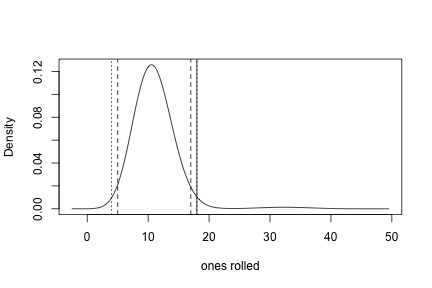
\includegraphics{flat-pps} \end{kframe}}
\end{knitrout}

The red line is our observation, which falls outside the 0.95 (dashed) density interval and right on the edge of the 0.97 (dotted) interval. 

Even assuming the high posterior probability given to fairness in the ``two model'' Bayesian test, the observation is an extereme event. 
Our high posterior simply owes to the fact that our observation would be {\em much more unlikely} if the die were loaded to even odds of rolling a one.

To construct a more direct Bayesian analogue of the NHST, we could proceed by calculating the posterior assuming a flat prior over all possible models. 
This distribution should have a peak at $\tfrac{18}{65}$, but it's width could  help inform our final decision.

\begin{knitrout}
\definecolor{shadecolor}{rgb}{.97, .97, .97}{\color{fgcolor}\begin{kframe}
\begin{flushleft}
\ttfamily\noindent
\hlsymbol{pri}{\ }\hlassignement{\usebox{\hlnormalsizeboxlessthan}-}{\ }\hlfunctioncall{rep}\hlkeyword{(}\hlnumber{1}\hlkeyword{/}\hlnumber{1000}\hlkeyword{,}{\ }\hlnumber{1000}\hlkeyword{)}\hspace*{\fill}\\
\hlstd{}\hlsymbol{mdls}{\ }\hlassignement{\usebox{\hlnormalsizeboxlessthan}-}{\ }\hlfunctioncall{seq}\hlkeyword{(}\hlnumber{0}\hlkeyword{,}{\ }\hlnumber{1}\hlkeyword{,}{\ }\hlargument{length.out}{\ }\hlargument{=}{\ }\hlnumber{1000}\hlkeyword{)}\hspace*{\fill}\\
\hlstd{}\hlsymbol{lik}{\ }\hlassignement{\usebox{\hlnormalsizeboxlessthan}-}{\ }\hlfunctioncall{dbinom}\hlkeyword{(}\hlsymbol{die.succ}\hlkeyword{,}{\ }\hlsymbol{die.trials}\hlkeyword{,}{\ }\hlargument{prob}{\ }\hlargument{=}{\ }\hlsymbol{mdls}\hlkeyword{)}\hspace*{\fill}\\
\hlstd{}\hlsymbol{post}{\ }\hlassignement{\usebox{\hlnormalsizeboxlessthan}-}{\ }\hlsymbol{pri}{\ }\hlkeyword{*}{\ }\hlsymbol{lik}\hspace*{\fill}\\
\hlstd{}\hlsymbol{post}{\ }\hlassignement{\usebox{\hlnormalsizeboxlessthan}-}{\ }\hlsymbol{post}\hlkeyword{/}\hlfunctioncall{sum}\hlkeyword{(}\hlsymbol{post}\hlkeyword{)}\hspace*{\fill}\\
\hlstd{}\hlfunctioncall{plot}\hlkeyword{(}\hlsymbol{post}{\ }\hlkeyword{\urltilda{}}{\ }\hlsymbol{mdls}\hlkeyword{,}{\ }\hlargument{type}{\ }\hlargument{=}{\ }\hlstring{"l"}\hlkeyword{,}{\ }\hlargument{xlab}{\ }\hlargument{=}{\ }\hlstring{"models"}\hlkeyword{,}{\ }\hlargument{ylab}{\ }\hlargument{=}{\ }\hlstring{"posterior"}\hlkeyword{)}\hspace*{\fill}\\
\hlstd{}\hlfunctioncall{abline}\hlkeyword{(}\hlargument{v}{\ }\hlargument{=}{\ }\hlnumber{1}\hlkeyword{/}\hlnumber{6}\hlkeyword{,}{\ }\hlargument{col}{\ }\hlargument{=}{\ }\hlstring{"red"}\hlkeyword{)}\hspace*{\fill}\\
\hlstd{}\hlsymbol{hella.samples}{\ }\hlassignement{\usebox{\hlnormalsizeboxlessthan}-}{\ }\hlfunctioncall{sample}\hlkeyword{(}\hlsymbol{mdls}\hlkeyword{,}{\ }\hlargument{size}{\ }\hlargument{=}{\ }\hlnumber{1e+06}\hlkeyword{,}{\ }\hlargument{replace}{\ }\hlargument{=}{\ }\hlnumber{TRUE}\hlkeyword{,}\hspace*{\fill}\\
\hlstd{}{\ }{\ }{\ }{\ }\hlargument{prob}{\ }\hlargument{=}{\ }\hlsymbol{post}\hlkeyword{)}\hspace*{\fill}\\
\hlstd{}\hlfunctioncall{abline}\hlkeyword{(}\hlargument{v}{\ }\hlargument{=}{\ }\hlfunctioncall{HPDI}\hlkeyword{(}\hlsymbol{hella.samples}\hlkeyword{,}{\ }\hlnumber{0.95}\hlkeyword{)}\hlkeyword{,}{\ }\hlargument{lty}{\ }\hlargument{=}{\ }\hlnumber{2}\hlkeyword{)}\hspace*{\fill}\\
\hlstd{}\hlfunctioncall{abline}\hlkeyword{(}\hlargument{v}{\ }\hlargument{=}{\ }\hlfunctioncall{HPDI}\hlkeyword{(}\hlsymbol{hella.samples}\hlkeyword{,}{\ }\hlnumber{0.99}\hlkeyword{)}\hlkeyword{,}{\ }\hlargument{lty}{\ }\hlargument{=}{\ }\hlnumber{3}\hlkeyword{)}\mbox{}
\normalfont
\end{flushleft}
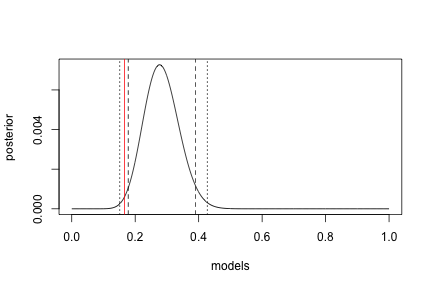
\includegraphics{flat-check} \end{kframe}}
\end{knitrout}

The red is a fair die, which falls between the 0.95 (dashed) and 0.99 (dotted) HPDI intervals. 
This procedure suggests that the posterior probability of fairness is rather low. 

Overall, the above results show that our assumptions about the prior and number of models are influencing the results of our tests.
This suggest we have insufficient data to conclude one way or another on the fairness of the die. 
If possible, we should attempt to collect more data. 

Of course, if we have very strong reasons to assume only two models, then we should still conclude the die is fair. 
For example, if we know that the only type of loaded die widely manufactured has even odds of rolling a one \dots 

\subsection*{Problem 3}
\label{problem3}

Our null, $H_0$ is that the die is fair. 
We want to compute the value of $Pr(fair)$ such that

\[
Pr( fair | data)  = \frac{Pr(data | fair)Pr(fair)}{Pr(data|fair)Pr(fair)+ Pr(data|loaded)Pr(loaded)} = 0.017
\]

(Our $p$ value from Problem 2(a).)

Both $Pr(fair)$ and $Pr(loaded)$ are unknown, but sum to unity. 
Multiplying through by the denominator and simplyfying to solve for $Pr(fair)$ \dots

\begin{align*}
&Pr(fair) Pr(data | fair) = 0.017 \cdot \left(Pr(data|fair)Pr(fair)+ Pr(data|loaded)(1-Pr(fair))\right)\\
 &\implies Pr(fair) \left[ Pr(data|fair) \cdot (1 - 0.017) + 0.017 \cdot Pr(data|loaded)\right] = 0.017 \cdot Pr(data|loaded)\\
 &\implies Pr(fair) = \frac{0.017 \cdot Pr(data|loaded)}{\left[ Pr(data|fair) \cdot (1 - 0.017) + 0.017 \cdot Pr(data|loaded)\right]}
\end{align*}


\begin{knitrout}
\definecolor{shadecolor}{rgb}{.97, .97, .97}{\color{fgcolor}\begin{kframe}
\begin{flushleft}
\ttfamily\noindent
\hlsymbol{pr.fair.pval}{\ }\hlassignement{\usebox{\hlnormalsizeboxlessthan}-}{\ }\hlsymbol{pd.pval}{\ }\hlkeyword{*}{\ }\hlsymbol{pr.data\usebox{\hlnormalsizeboxunderscore}loaded}\hlkeyword{/}\hlkeyword{(}\hlsymbol{pr.data\usebox{\hlnormalsizeboxunderscore}fair}{\ }\hlkeyword{*}\hspace*{\fill}\\
\hlstd{}{\ }{\ }{\ }{\ }\hlkeyword{(}\hlnumber{1}{\ }\hlkeyword{-}{\ }\hlsymbol{pd.pval}\hlkeyword{)}{\ }\hlkeyword{+}{\ }\hlsymbol{pd.pval}{\ }\hlkeyword{*}{\ }\hlsymbol{pr.data\usebox{\hlnormalsizeboxunderscore}loaded}\hlkeyword{)}\hspace*{\fill}\\
\hlstd{}\hlsymbol{pr.fair.pval}\mbox{}
\normalfont
\end{flushleft}
\begin{verbatim}
## [1] 0.0002584
\end{verbatim}
\end{kframe}}
\end{knitrout}


Thus, the prior probabilty of the null must be {\em very, very} low $Pr(H_0 | Data) = 2.6\times10^{-4}$ to obtain a prior probability equal to the $p$ value from above.

\begin{knitrout}
\definecolor{shadecolor}{rgb}{.97, .97, .97}{\color{fgcolor}\begin{kframe}
\begin{flushleft}
\ttfamily\noindent
\hlsymbol{post.check}{\ }\hlassignement{\usebox{\hlnormalsizeboxlessthan}-}{\ }\hlsymbol{pr.fair.pval}{\ }\hlkeyword{*}{\ }\hlsymbol{pr.data\usebox{\hlnormalsizeboxunderscore}fair}\hlkeyword{/}\hlkeyword{(}\hlsymbol{pr.data\usebox{\hlnormalsizeboxunderscore}fair}{\ }\hlkeyword{*}\hspace*{\fill}\\
\hlstd{}{\ }{\ }{\ }{\ }\hlsymbol{pr.fair.pval}{\ }\hlkeyword{+}{\ }\hlsymbol{pr.data\usebox{\hlnormalsizeboxunderscore}loaded}{\ }\hlkeyword{*}{\ }\hlkeyword{(}\hlnumber{1}{\ }\hlkeyword{-}{\ }\hlsymbol{pr.fair.pval}\hlkeyword{)}\hlkeyword{)}\hspace*{\fill}\\
\hlstd{}\hlsymbol{post.check}\mbox{}
\normalfont
\end{flushleft}
\begin{verbatim}
## [1] 0.01752
\end{verbatim}
\end{kframe}}
\end{knitrout}





\subsection*{Colophon}

\begin{knitrout}
\definecolor{shadecolor}{rgb}{.97, .97, .97}{\color{fgcolor}\begin{kframe}
\begin{flushleft}
\ttfamily\noindent
\hlfunctioncall{require}\hlkeyword{(}\hlsymbol{knitr}\hlkeyword{)}{\ }{\ }\hlcomment{\usebox{\hlnormalsizeboxhash}\usebox{\hlnormalsizeboxhash}\usebox{\hlnormalsizeboxhash}{\ }the{\ }package}\hspace*{\fill}\\
\hlstd{}\hlfunctioncall{knit}\hlkeyword{(}\hlstring{"/Users/jaime/PHD/stat-rethink/hw2ashander.Rnw"}\hlkeyword{)}{\ }{\ }\hlcomment{\usebox{\hlnormalsizeboxhash}\usebox{\hlnormalsizeboxhash}{\ }to{\ }run}\mbox{}
\normalfont
\end{flushleft}
\end{kframe}}
\end{knitrout}



\end{document}
